\documentclass[../mainfile.tex]{subfiles}
\RequirePackage[nosumlimits]{amsmath} %Preiset den Mathmode
\RequirePackage{ngerman} %Ich mag Deutsch
\usepackage{graphicx} %Hab Bild
\RequirePackage[utf8x]{inputenc} %Mehr Deutsch
\graphicspath{ {img/} } %Path zum Bild
\usepackage{tabularx} %Für die sch*** Tabelle, damit sie centered ist

\begin{document}
	\subsection{Extremwertaufgaben}
		\def\tabularxcolumn#1{m{#1}}
		\begin{tabularx}{\textwidth}{ | X | X |}
			\hline
			Beispiel & Theorie \\
			\hline 
			An eine Mauer soll mit 20m Maschendrahtzaun ein rechteckiges Areal begrenzt werden, sodass das Areal möglichst Flächengroß ist. Wie sind die Maße zu wählen? &  \underline{Angabe} \\
			\hline 
			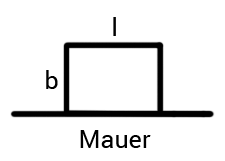
\includegraphics[scale=0.4]{diff1_009_01.png} & \underline{Skizze} \\
			\hline
			\begin{gather*}
			A \rightarrow Max \\
			A(l, b) = b \cdot l
			\end{gather*}
			 &  Hauptbedingung aufstellen(HB)\\
			\hline
			\[2b+l=20\] & Nebenbedingung aufstellen (NB) \\
			\hline
			\begin{gather*}
			l = 20 - 2b \\
			A(b) = b(20-2b) \\
			A(b) = 20b - 2b^2  
			\end{gather*} & Nebenbedingung in Hauptbedingung einsetzen (NB $\rightarrow$ HB) \\
			\hline
			\begin{gather*}
			A'(b) = 20-4b \\
			A''(b)=-4
			\end{gather*} & Ableiten \\
		 	\hline
		 	\begin{gather*} 
		 	A'(b) = 0 \\
		 	0 = 20-4b \\
		 	\Longrightarrow b = 5 \\
		 	A''(b) < 0 \\
		 	\Longrightarrow b = 5 \text{ Maximum}
		 	\end{gather*} & Extremstellen bestimmen \\
		 	\hline
		 \end{tabularx}
	 	 \begin{tabularx}{\textwidth}{ | X | X |}
			\hline 
		 	$l = 20 - 2 \cdot 5 = 10$ & Andere Variable berechnen \\
		 	\hline
		 	/ & Randwerte betrachten \\
		 	\hline
		 	Das ideal an die Mauer angelehnte Areal besitzt die Maße 10x5. & Antwort \\
		 	\hline

		\end{tabularx}
\end{document}